\documentclass{exam}

\usepackage{indentfirst}
\usepackage{graphicx}
\usepackage{listings}
\usepackage{color}
\usepackage{fancyvrb}
\usepackage{amsmath}
\usepackage{amssymb}

\definecolor{mygreen}{rgb}{0,0.6,0}
\definecolor{mygray}{rgb}{0.5,0.5,0.5}
\definecolor{mymauve}{rgb}{0.58,0,0.82}

\lstset{ %
	backgroundcolor=\color{white},		% choose the background color; you must add \usepackage{color} or \usepackage{xcolor}
	basicstyle=\small\ttfamily,		% the size of the fonts that are used for the code
	breakatwhitespace=false,			% sets if automatic breaks should only happen at whitespace
	breaklines=true,					% sets automatic line breaking
	captionpos=b,						% sets the caption-position to bottom
	columns=fullflexible,
	commentstyle=\color{mygreen},		% comment style
	deletekeywords={...},				% if you want to delete keywords from the given language
	escapeinside={\%*}{*)},			% if you want to add LaTeX within your code
	extendedchars=true,				% lets you use non-ASCII characters; for 8-bits encodings only, does not work with UTF-8
	frame=single,						% adds a frame around the code
	keepspaces=true,					% keeps spaces in text, useful for keeping indentation of code (possibly needs columns=flexible)
	keywordstyle=\color{blue},			% keyword style
	language=Octave,					% the language of the code
	morekeywords={*,...},				% if you want to add more keywords to the set
	%   numbers=left,						% where to put the line-numbers; possible values are (none, left, right)
	%   numbersep=6pt,						% how far the line-numbers are from the code
	%   numberstyle=\tiny\color{mygray},	% the style that is used for the line-numbers
	rulecolor=\color{black},			% if not set, the frame-color may be changed on line-breaks within not-black text (e.g. comments (green here))
	showspaces=false,					% show spaces everywhere adding particular underscores; it overrides 'showstringspaces'
	showstringspaces=false,			% underline spaces within strings only
	showtabs=false,					% show tabs within strings adding particular underscores
	stepnumber=1,						% the step between two line-numbers. If it's 1, each line will be numbered
	stringstyle=\color{mymauve},		% string literal style
	tabsize=2,							% sets default tabsize to 2 spaces
	title=\lstname						% show the filename of files included with \lstinputlisting; also try caption instead of title
}

\newcommand{\octavescript}[2]{
	\lstinputlisting[caption=#2,label=#1]{#1}
}

\newcommand{\MNLab}{Laborator\ \#11}
\newcommand{\MNLabTitle}{Derivare numerică. Metode Newton-Cotes.}
\newcommand{\MNLabTitleHeader}{Derivare numerică}
\newcommand{\MNAuthor}{Andrei Stan, Radu Poenaru, Radu Constantinescu}

\renewcommand{\contentsname}{Cuprins}
\renewcommand{\figurename}{Figura}

\setlength{\parskip}{0.5\baselineskip}

\graphicspath{{./img/}}

\title{
	\textmd{\textbf{\MNLabTitle}}
	\author{Colaboratori: \MNAuthor}
}

\pagestyle{headandfoot}

\header{Metode Numerice}
{\MNLabTitleHeader, Pagina \thepage\ din \numpages}
{2025}
\footer{Facultatea de Automatică și Calculatoare}{}{Pagina \thepage\ din \numpages}

\begin{document}

\begin{coverpages}

	\maketitle
	\tableofcontents

\end{coverpages}

\section{Obiective laborator}

În urma parcurgerii acestui laborator, studentul va fi capabil să:
\begin{itemize}
	\item
	      utilizeze metodele de derivare \c{s}i integrare numeric\u{a} prezentate;
	\item
	      \^{i}n\c{t}eleag\u{a} diferen\c{t}ele între diferitele versiuni ale acestor metode;
	\item
	      situa\c{t}iile \^{i}n care aceste metode sunt potrivite.
\end{itemize}

\section{No\c{t}iuni teoretice}
Ne propunem s\u{a} calcul\u{a}m, \^{i}n mod aproximativ, valorile $I[f]=\int\limits_{a}^{b}f(x)dx$ \c{s}i $D[f]=f^{(p)}(x_0)$, \^{i}n condi\c{t}iile \^{i}n care:
\begin{itemize}
	\item func\c{t}ia $f$ este continu\u{a} pe intervalul [a, b];
	\item primitiva $F$ nu este cunoscut\u{a};
	\item func\c{t}ia $f$ este cunoscut\u{a} numai prin valorile $f(x_i)$, într-un num\u{a}r restr\^{a}ns de puncte $x_i$, $i = 0 : N.$
\end{itemize}

\subsection{Derivare numeric\u{a}}

\^{I}ntruc\^{a}t derivata func\c{t}iei $f$ \^{i}n punctul $x_0$ este definit\u{a} ca
$$f'(x_0)=\lim\limits_{h\rightarrow0}\frac{f(x_0+h)-f(x_0)}{h},$$
un mod evident de a aproxima $f'(x_0)$ este calculul
$$\frac{f(x_0+h)-f(x_0)}{h},$$
pentru valori mici ale lui $h$.

Vom analiza eroarea ob\c{t}inut\u{a} prin aceast\u{a} metod\u{a}, cu ajutorul polinomului de interpolare Lagrange de grad 1, cunosc\^{a}nd valorile func\c{t}iei \^{i}n punctele $x_0$ \c{s}i $x_1=x_0+h$. Consider\u{a}m $f\in C^2[a, b]$ şi $x_0, x_1 \in [a, b].$

$$f(x)=P_1(x)+\frac{(x-x_0)(x-x_1)}{2!}f''(\xi(x))$$
$$f(x)=\frac{f(x_0)(x-x_0-h)}{-h}+\frac{f(x_0+h)(x-x_0)}{h}+\frac{(x-x_0)(x-x_1)}{2}f''(\xi(x)), \quad
	\xi(x)\in[a, b]$$

Deriv\^{a}nd, se ajunge la
$$f'(x)=\frac{f(x_0+h)-f(x_0)}{h}+D_x\left[\frac{(x-x_0)(x-x_0-h)}{2}f''(\xi(x))\right]$$ $$=\frac{f(x_0+h)-f(x_0)}{h}+\frac{2(x-x_0)-h}{2}f''(\xi(x))+\frac{(x-x_0)(x-x_0-h)}{2}D_x(f''(\xi(x))).$$

Astfel, $$f'(x)\approx\frac{f(x_0+h)-f(x_0)}{h},$$
cu eroarea
$$\frac{2(x-x_0)-h}{2}f''(\xi(x))+\frac{(x-x_0)(x-x_0-h)}{2}D_x(f''(\xi(x))).$$

Pentru $x=x_0$, formula se simplific\u{a} astfel (two-point formula):
$$f'(x_0)=\frac{f(x_0+h)-f(x_0)}{h}-\frac{h}{2}f''(\xi), \xi \in [x_0, x_0+h].$$

\begin{figure}[ht]
	\begin{center}
		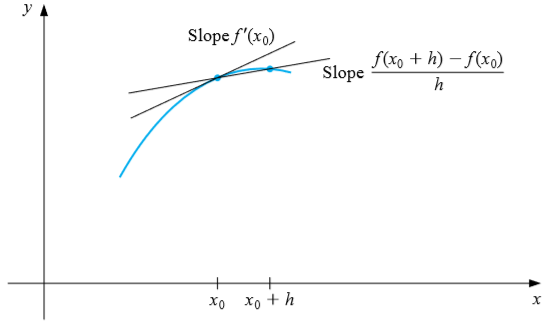
\includegraphics[width=0.5\columnwidth]{./img/d_simple}
		\caption{Interpretare geometrică pentru formula de derivare two-point.}
	\end{center}
\end{figure}

Aplic\^{a}nd o tehnic\u{a} similar\u{a}, dar folosind polinomul Lagrange de grad 2, cunosc\^{a}nd valorile func\c{t}iei \^{i}n punctele $x_0, x_0+h, x_0+2h$ \c{s}i consider\^{a}nd c\u{a} exist\u{a} $f'''$ pe un interval ce con\c{t}ine aceste abscise, ob\c{t}inem (three-point endpoint formula):
$$f'(x_0)=\frac{1}{2h}[-3f(x_0)+4f(x_0+h)-f(x_0+2h)]+\frac{h^2}{3}f'''(\xi), \xi \in [x_0, x_0+2h].$$

Aceast\u{a} formul\u{a} este util\u{a} pentru aproximarea derivatei la cap\u{a}tul unui interval (ex: $x_0$), situa\c{t}ie ce apare, spre exemplu, la interpol\u{a}rile cu spline-uri cubice tensionate.

Pentru aproximarea derivatei unei func\c{t}ii \^{i}ntr-un punct interior unui interval, este recomandat\u{a} folosirea urm\u{a}toarei formule (ob\c{t}inut\u{a} cu ajutorul polinomului de interpolare Lagrange de grad 2, \^{i}n punctele $x_0-h$, $x_0$, $x_0+h$ (three-point midpoint formula):
$$f'(x_0)=\frac{1}{2h}\left[f(x_0+h)-f(x_0-h)\right]-\frac{h^2}{6}f'''(\xi), \xi \in [x_0-h, x_0+h].$$

\begin{figure}[ht]

	\begin{center}
		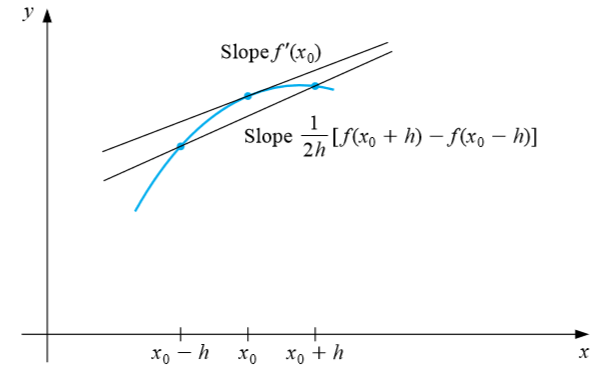
\includegraphics[width=0.5\columnwidth]{./img/d_three}
		\caption{Interpretare geometrică pentru formula de derivare three-point midpoint.}
	\end{center}
\end{figure}

\subsubsection{Observaţie}

\^{I}n tehnicile de derivare numeric\u{a}, reducerea pasului $h$ duce la reducerea erorii teoretice, îns\u{a} cu costul cre\c{s}terii erorilor de rotunjire. Pentru a ilustra acest comportament, vom examina formula:
$$f'(x_0)=\frac{1}{2h}\left[f(x_0+h)-f(x_0-h)\right]-\frac{h^2}{6}f'''(\xi), \xi \in [x_0-h, x_0+h].$$

Dac\u{a} \^{i}n evalu\u{a}rile $f(x_0+h)$ \c{s}i $f(x_0-h)$ apar erorile $\epsilon_+$ \c{s}i $\epsilon_-$, not\^{a}nd cu $\tilde{f}(x_0+h)$ \c{s}i $\tilde{f}(x_0-h)$ valorile calculate efectiv, avem rela\c{t}iile:
$$f(x_0+h) = \tilde{f}(x_0+h)+\epsilon_+$$
$$f(x_0-h) = \tilde{f}(x_0-h)+\epsilon_-$$

Astfel, presupun\^{a}nd c\u{a} erorile $\epsilon_+$ \c{s}i $\epsilon_-$ sunt m\u{a}rginite de $\epsilon>0$ \c{s}i c\u{a} $f'''$ este marginit\u{a} de $M>0$, eroarea total\u{a} a aproxim\u{a}rii devine:
$$\left|f'(x_0) -\frac{\tilde{f}(x_0+h)-\tilde{f}(x_0-h)}{2h}\right|\leq\frac{\epsilon}{h}+\frac{h^2}{6}M.$$

Pentru a reduce termenul $\frac{h^2}{6}M$ este necesar\u{a} reducerea lui $h$, care duce \^{i}ns\u{a} la cre\c{s}terea termenului $\frac{\epsilon}{h}$ (specific erorii de rotunjire), acest termen ajung\^{a}nd s\u{a} domine calculele.

\subsection{Integrare numeric\u{a}}

Definim o metod\u{a} aproximativ\u{a} de integrare astfel:
$$I_N[f]=\sum\limits_{i=0}^{N}A_{i}f(x_{i}).$$

O astfel de metod\u{a} este convergent\u{a} dac\u{a}:
$$\lim\limits_{N\rightarrow \infty} \left|I[f]-I_N[f]\right|=0.$$

\subsubsection{Metode Newton-Cotes}

Pentru o formul\u{a} de integrare aproximativ\u{a} putem scrie
$$\int\limits_{a}^{b}f(x)w(x)dx=\sum\limits_{i=0}^{N}A_{i}f(x_{i})+R_N.$$

\^{I}n metodele de tip Newton-Cotes, abscisele $x_{i}$ se aleg echidistante \^{i}n intervalul $[a, b]$
$$x_{i}=a+i\frac{(b-a)}{N}, i=0:N.$$

Coeficien\c{t}ii $A_{i}$ se determin\u{a} impun\^{a}nd ca formula aproximativ\u{a} s\u{a} fie exact\u{a} ($R_N=0$) dac\u{a} $f$ apar\c{t}ine unei anumite clase de func\c{t}ii (de exemplu, polinoame de grad $\leq N$). Astfel, vom aproxima func\c{t}ia prin polinomul ei de interpolare Lagrange
$$P_N(x) = \sum\limits_{i=0}^{N}f(x_i)l_i(x),  \quad l_i(x) = \prod\limits_{j=0, j \neq i}^{N}\frac{(x-x_j)}{(x_i-x_j)}.$$

\^{I}n acest fel, ob\c{t}inem $A_i=\int\limits_{a}^{b}l_i(x)w(x)dx$.

Deoarece eroarea polinomului de interpolare respect\u{a} $\left|f(x)-P_N(x)\right|\leq\frac{\left|f^{(N+1)}(\xi)\right|}{(N+1)!}\left|(x-x_0) ... (x-x_N)\right|$, cu $\xi\in[a, b]$, prin integrare ob\c{t}inem expresia erorii \^{i}n metodele Newton-Cotes:
$$R_N\leq\frac{\left|f^{(N+1)}(\xi)\right|}{(N+1)!}\int\limits_{a}^{b}\left|(x-x_0) ... (x-x_N)\right|w(x)dx.$$

Datorit\u{a} instabilit\u{a}\c{t}ii interpol\u{a}rii polinomiale se folosesc polinoame de interpolare de grad mic.

Astfel, pentru $N=1$ se ob\c{t}ine \textit{formula trapezelor}:
$$\int\limits_{a}^{b}f(x)dx=\frac{h}{2}\left[f(a)+f(b)\right]-\frac{h^3f''(\xi)}{12}, \quad h = b-a.$$

\begin{figure}[ht]

	\begin{center}
		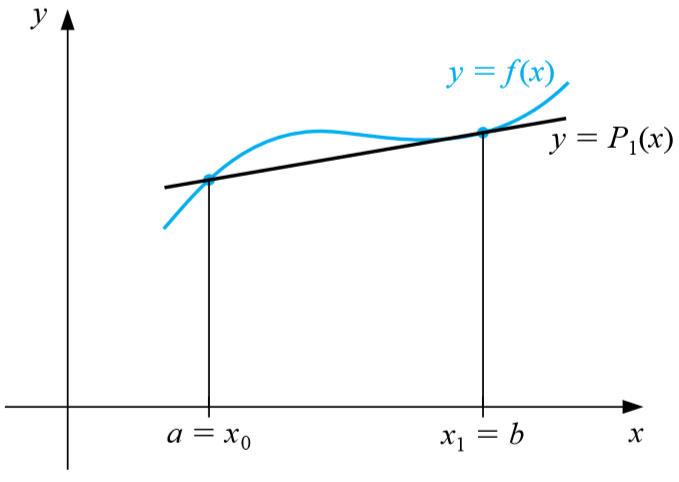
\includegraphics[width=0.5\columnwidth]{./img/trapez}
		\caption{Interpretare geometrică pentru formula trapezelor.}
	\end{center}
\end{figure}


Pentru $N=2$, se ob\c{t}ine \textit{formula Simpson} (Figure 2):
$$\int\limits_{a}^{b}f(x)dx=\frac{h}{3}\left[f(a)+4f\left(\frac{a+b}{2}\right)+f(b)\right]-\frac{h^5f^{(4)}(\xi)}{90}, \quad h=b-a.$$

\begin{figure}[ht]

	\begin{center}
		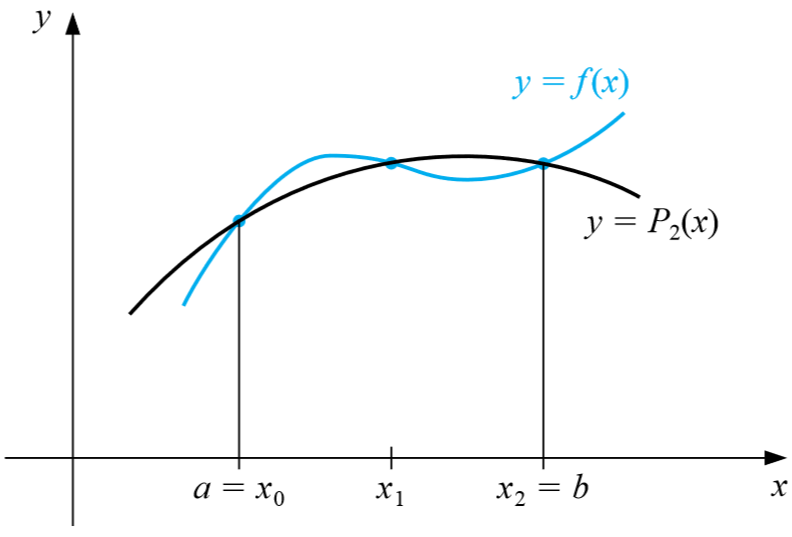
\includegraphics[width=0.5\columnwidth]{./img/simpson}
		\caption{Interpretare geometrică pentru formula Simpson.}
	\end{center}
\end{figure}
Aceste formule folosesc pu\c{t}ine puncte, ceea ce ne determin\u{a} s\u{a} aproxim\u{a}m integrala ca o sum\u{a} de integrale calculate pe intervale mai mici
$$\int\limits_{x_0}^{x_N}f(x)dx=\int\limits_{x_0}^{x_1}f(x)dx+...+\int\limits_{x_{N-1}}^{x_{N}}f(x)dx.$$

Astfel, ob\c{t}inem:

\begin{itemize}
	\item \textit{formula compus\u{a} a trapezelor}
	      $$\int\limits_{a}^{b}f(x)dx\approx\frac{h}{2}\left[f(a)+f(b)+2\sum\limits_{i=1}^{N-1}f(a+ih)\right], \quad h = \frac{(b-a)}{N}$$

	      \begin{figure}[ht]

		      \begin{center}
			      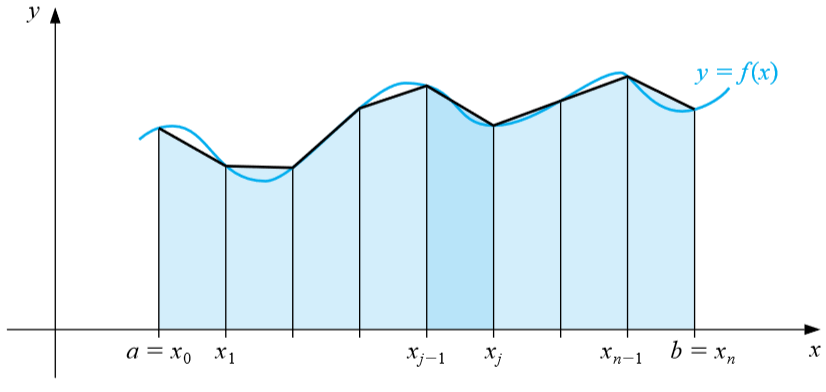
\includegraphics[width=0.5\columnwidth]{./img/c_trapez}
			      \caption{Interpretare geometrică pentru formula  compus\u{a} a trapezelor.}
		      \end{center}
	      \end{figure}

	\item \textit{formula compus\u{a} Simpson}
	      $$\int\limits_{a}^{b}f(x)dx\approx\frac{h}{3}\left[f(a)+f(b)+4\sum\limits_{i=1}^{N/2}f(x_{2i-1})+2\sum\limits_{i=1}^{N/2-1}f(x_{2i})\right], \quad h = \frac{(b-a)}{N}, x_i=a+ih$$

	      \begin{figure}[ht]

		      \begin{center}
			      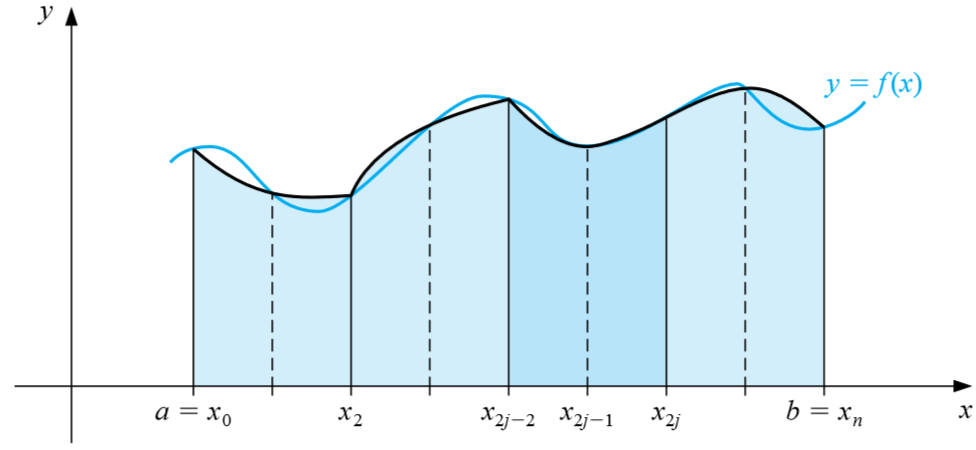
\includegraphics[width=0.5\columnwidth]{./img/c_simpson}
			      \caption{Interpretare geometrică pentru formula compus\u{a} Simpson.}
		      \end{center}
	      \end{figure}

\end{itemize}


\section{Probleme rezolvate}

\subsection{Problema 1}
a) Folosind formula de derivare two-point, aproxima\c{t}i derivata func\c{t}iei $f(x)=sin(x)$ \^{i}n punctele $x_0=0.2$, $x_1=0.5$, $x_2=0.9$.

b) Calcula\c{t}i eroarea de aproximare \^{i}n punctul $x_{0} = 0.5$ \c{s}i g\u{a}si\c{t}i o margine superioar\u{a} teoretic\u{a} pentru aceasta folosind formula erorii.

\textit{Solu\c{t}ie}: a)

\octavescript{./src/lab11Pr1.m}{Metoda de derivare two-point.}

\begin{center}
	\begin{tabular}{| l | l |}
		\hline
		\textbf{Date de intrare:} & \textbf{Date de ieşire:} \\
		$@sin,$
		$xi = $
		$
			\begin{bmatrix}
				0.2 \\
				0.5 \\
				0.9 \\
			\end{bmatrix}
		$
		                          &
		$diffs = $
		$
			\begin{bmatrix}
				0.93585 \\
				0.79310 \\
				0.79310 \\
			\end{bmatrix}
		$
		\\
		\hline
	\end{tabular}
\end{center}

b)
\^{I}n punctul $x_0=0.5$, eroarea de aproximare este $Err=cos(0.5)-diffs(1) = 0.025$.

\^{I}n punctul $x_0=0.5$, pentru formula utilizat\u{a}, forma erorii este $\left|Err(\xi)\right| = \left|\frac{h}{2}f''(\xi)\right|=\left|0.05\cdot sin(\xi)\right|$, cu $\xi\in\left[0.5,0.6\right]\Rightarrow \max\limits_{\xi\in\left[0.5,0.6\right]}Err(\xi)=\max\limits_{\xi\in\left[0.5,0.6\right]}0.05\cdot sin(\xi)=0.05\cdot sin(0.6)=0.0282$. Se verific\u{a} faptul c\u{a} marginea teoretic\u{a} \^{i}ncadreaz\u{a} eroarea efectiv\u{a} \^{i}n acest caz.

%\end{Problem}

\subsection{Problema 2}
a) Scrie\c{t}i dou\u{a} func\c{t}ii OCTAVE care calculeaz\u{a} derivata unei func\c{t}ii \^{i}ntr-un punct $x_0$ dat, folosind formulele three-point midpoint, respectiv three-point endpoint. $fx$ este un vector ce con\c{t}ine valorile func\c{t}iei  \^{i}n punctele necesare fiec\u{a}rei metode.

b) Folosi\c{t}i aceste func\c{t}ii pentru a completa tabelul ($f(x)=e^{3x}$):
$$
	\begin{tabular}{ c | c | c }
		x   & f(x)    & f'(x) \\
		\hline
		2.3 & 992.27  &       \\
		2.5 & 1808.04 &       \\
		2.7 & 3294.47 &       \\
	\end{tabular}
$$
\textit{Solu\c{t}ie}:./

\octavescript{./src/DMid.m}{Metoda de derivare three-point midpoint.}
\octavescript{./src/DEnd.m}{Metoda de derivare  three-point endpoint.}
\octavescript{./src/lab11Pr2.m}{lab11Pr2.m.}

\begin{center}
	\begin{tabular}{| l | l |}
		\hline
		\textbf{Date de intrare:} & \textbf{Date de ieşire:} \\
		$f\_e3x,$
		$xi = $
		$
			\begin{bmatrix}
				2.3 \\
				2.5 \\
				2.7 \\
			\end{bmatrix}
		$
		                          &
		$diffs = $
		$
			\begin{bmatrix}
				2402.2  \\
				5755.5  \\
				-9108.8 \\
			\end{bmatrix}
		$
		\\
		\hline
	\end{tabular}
\end{center}

unde  $f\_e3x=@(x)$  $e.\char`^(3*x).$
%\end{Problem}


\subsection{Problema 3}
a)	Folosind formula compus\u{a} Simpson pentru N = 4, aproxima\c{t}i integrala $\int\limits_{3}^{5}xlog(x)dx.$

b) 	 Folosind formula compus\u{a} a trapezelor pentru N = 4, aproxima\c{t}i integrala $\int\limits_{1}^{3}e^{3x} dx.$

\textit{Solu\c{t}ie}:
\octavescript{./src/compositeSimpson.m}{Formula compus\u{a} Simpson.}
\octavescript{./src/compositeTrapezoidal.m}{Formula compus\u{a} a trapezelor.}
\octavescript{./src/lab11Pr3.m}{lab11Pr3.m.}

\begin{center}
	\begin{tabular}{| l | l |}
		\hline
		\textbf{Date de intrare:} & \textbf{Date de ieşire:} \\
		$f\_xlogx, a=3,b= 5, N=4, @compositeSimpson$
		                          &
		$rez =11.174 $
		\\

		$f\_e3x, a=1, b=3, N=4, @compositeTrapezoidal$

		                          &
		$rez = 3181.5$
		\\

		\hline
	\end{tabular}
\end{center}

unde  $f\_xlogx=@(x)$  $x.*log(x)$, $f\_e3x=@(x)$  $e.\char`^(3*x).$

%\end{Problem}

\subsection{Problema 4}
Determina\c{t}i valoarea maxim\u{a} a lui $h=b-a,$ $b>a,$ astfel \^{i}nc\^{a}t aproximarea integralei $\int\limits_{a}^{b}\frac{1}{x+4}dx$, folosind metoda trapezelor, s\u{a} nu poat\u{a} avea o eroare mai mare decât $ 10^{-4}$, conform erorii din formul\u{a}. Se cunoa\c{s}te $a=1$.

\textit{Solu\c{t}ie}:
Aproxim\^{a}nd integrala dat\u{a} cu formula trapezelor, valoarea absolut\u{a} a erorii va avea forma

$$\left|Err(\xi)\right|=h^3\frac{\left|f''(\xi)\right|}{12}, \quad \xi\in[a,b].$$

Trebuie ca $\left|Err(\xi)\right| \leq 10^{-4},$ $ \forall\xi\in[a,b]\Rightarrow h^3\frac{\left|f''(\xi)\right|}{12}\leq 10^{-4}, \quad \forall\xi\in[a,b].$

Cum $f''(\xi)=\frac{2}{(x+4)^3}$ \c{s}i $a=1\Rightarrow \frac{h^3}{6}\frac{1}{(\xi+4)^3}\leq10^{-4},\quad $ $\forall\xi\in[1,b].$

Deoarece $\max\limits_{\xi\in\left[1,b\right]}\frac{1}{(\xi+4)^3}=\frac{1}{5^3}\Rightarrow \frac{h^3}{750}\leq 10^{-4}\Rightarrow h \leq 0.4217.$
%\end{Problem}


\section{Probleme propuse}

\subsection{Problema 1}
a)Aproxima\c{t}i integrala $ I=\int\limits_0^{\frac{\pi}{2}}\frac{sin(x)}{x}dx $ prin metoda Simpson folosind 3 puncte.

b) Se d\u{a} $f:[a,b]\times[c,d]\rightarrow\mathbb{R}$. Calcula\c{t}i $I=\int\limits_a^b\int\limits_c^df(x,y)dxdy.$
%\end{Problem}

\subsection{Problema 2}
Calcula\c{t}i pasul $h$ astfel \^{i}nc\^{a}t, aproxim\^{a}nd $\int\limits_0^{\frac{\pi}{2}}sin(x)dx$ prin metoda trapezelor, eroarea s\u{a} fie mai mic\u{a} dec\^{a}t $\varepsilon=\beta\cdot 10^{-t}$.
%\end{Problem}

\subsection{Problema 3}
Calcula\c{t}i aproximativ integrala $\int\limits_0^1ln(1+x^2)dx$, folosind formula compus\u{a} a trapezelor pentru $N=4$.
%\end{Problem}

\subsection{Problema 4}
Pentru formula de integrare de tip Newton-Cotes, $\int\limits_a^bf(x)w(x)dx\approx\sum\limits_{i=0}^{N}A_if(x_i)$, s\u{a} se arate c\u{a}  $a_i=\int\limits_a^bw(x)l_i(x)dx$, \^{i}n care $l_i$ reprezint\u{a} multiplicatorii din formula de interpolare Lagrange.
%\end{Problem}

\end{document}
